\documentclass{article}

\usepackage{amsfonts,graphicx}


\setlength{\textwidth}{17cm} \setlength{\textheight}{9in}
\oddsidemargin=-0.2cm \topmargin=-1.3cm
\renewcommand{\thesection}{\Alph{section}}
\renewcommand{\thepage}{\thesection-\arabic{page}}

\title{Collage Sculptures}

\author{Elizabeth Muhm}

\begin{document}


\maketitle



\begin{abstract}
In this proposal, I propose this and that. 
\end{abstract}



%%%%%%%%%%%%%%%%%%%%%%%%%%%%%%%%%%%%%%%%
%%%%%%%%%%%%%%%%%%%%%%%%%%%%%%%%%%%%%%%%
\section{Motivation and Introduction}

In the world of fine art, we see many examples of collage objects, one form made up of unique elements, such as in the paintings of Arcimboldo and the sculptures Heather Jansch.  The composite work takes on a new meaning derived from the form and composition of its elements.  Following suit, in the realm of computer graphics, artists have created 3D collage objects, often painstakingly modeling them by hand.  Fitting the elements together is a difficult challenge.  Here I propose an algorithm for automatically assembling elements into a target shape based on a (physically based?) gravitational pull toward center regions of a target shape.  The target space will be voxelized, and a distance function to the surface of the target object will be defined over this space.  Each element to be added to the final composite will be represented by a bounding sphere.  Each point in the space, represented by a voxel, will exert a force on the bounding sphere, pushing it into the form of the composite object.

\begin{figure}[htbp]
\begin{tabular}{cccccc}

\includegraphics[height=2.00in]{images/archimboldo}&
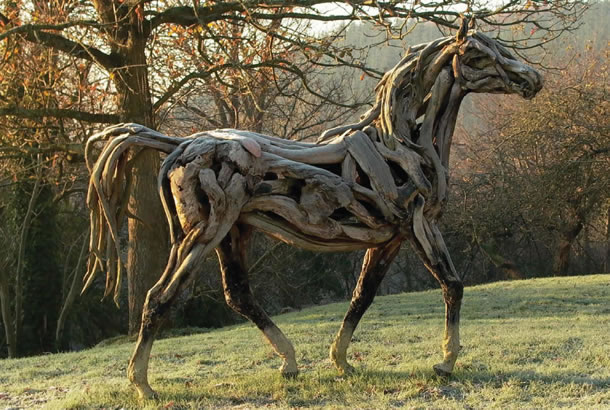
\includegraphics[height=2.00in]{images/jansch}&
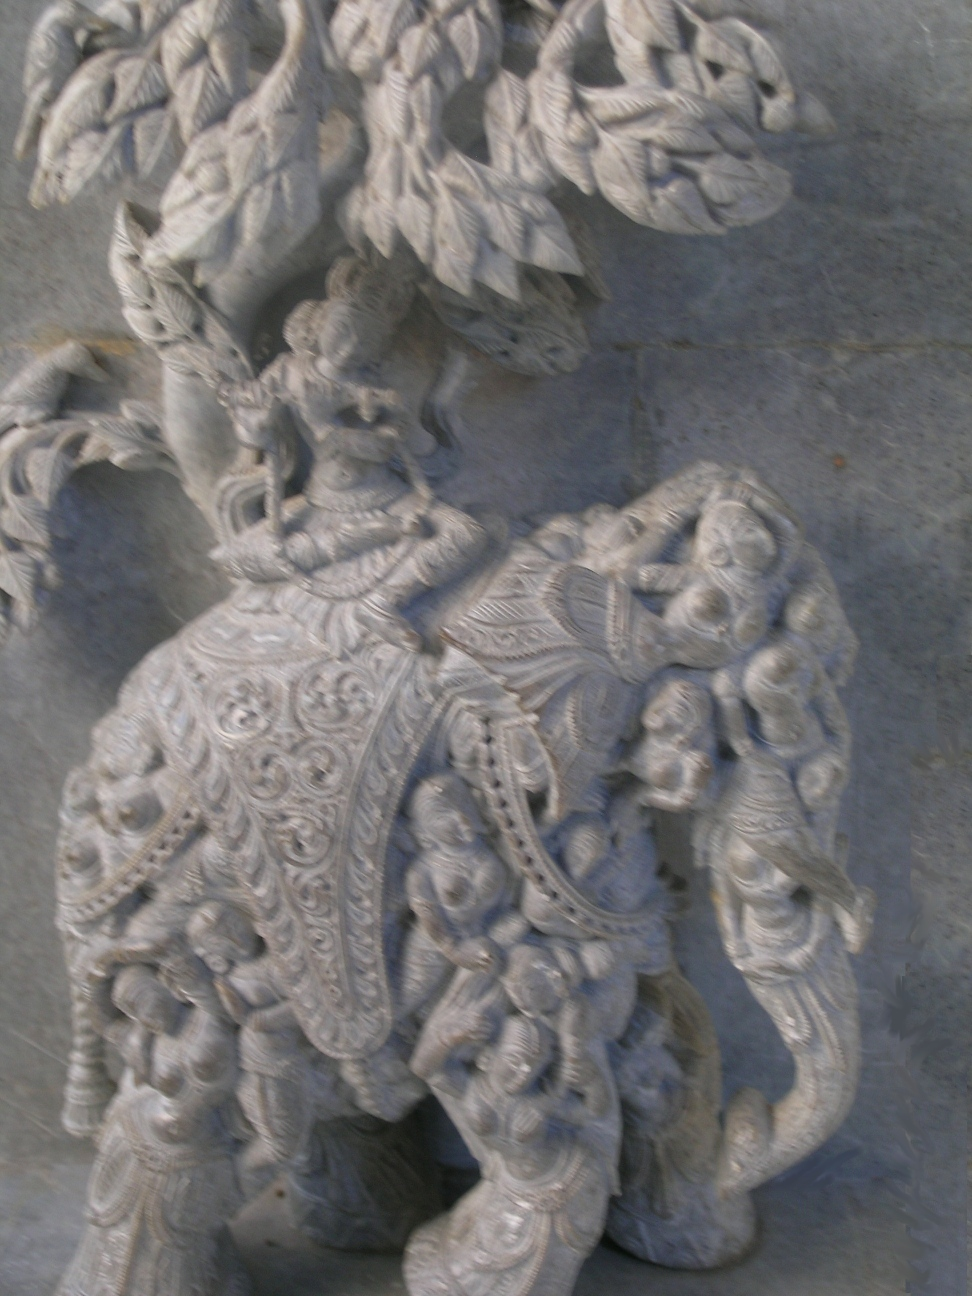
\includegraphics[height=2.00in]{images/elephant}\\
(a) Vertumnus, 1590 & (b) Apollo, 2005 \\
\end{tabular}
\caption{Examples of college art: (a) An example of collage images by Giuseppe Arcimboldo, (b) an example of collage sculpture by Heather Jansch.  (c) A collage sculpture from India. }
\label{fig:regions}
\end{figure}

\section{Background/Literature Review}

\cite{Kim2002}

Work has been done to create an art-directable algorithm to assemble 3D collages based on matching best fit shape descriptions for open spaces in a target shape  \cite{Gal2007}. I plan to apply a different approach that does not primarily use shape descriptors but instead relies on a gravity simulation and collisions to fill out a target shape with elements. Gal et al.'s algorithm gave high priority to the visibility of each individual element in order that the result is a "collage" rather than a "mosaic" in which the elements would be less distinct.  I hope to create denser collages in which the elements are still visible and distinct but more densely packed to better approximate the target shape.

To accommodate simulations with large numbers of elements colliding and settling together, I will use a method for setting interior objects to "sleep" so that those that are settled into the target shape are no longer simulated.  This method is based on the work of Hsu and Keyser who used it to build piles of elements that settle together \cite{Hsu2010}.

\section{Problem}

	
	The goal of this work is an algorithm that automatically assembles a collection of user-specified elements into a target shape subject to the following aesthetic rules.  First, the packing of the elements should be dense enough to convey the target shape.  Second, if the elements overlap at all, it will be very minimal.  Third, the algorithm will not alter the scale of the user-specified elements.  The algorithm will allow a limited degree of art direction as users will be able to set the initial position of elements if they choose, as well as reset individual elements in the simulation.

\section{Method}

	
	Preliminary work suggests this approach of using a gravity simulation to assemble objects into a target shape will produce dense packing.  In this test, uniform sphere elements assembled into a larger, target sphere.  A gravity force directed at the center of the target sphere pulled the elements.  A large amount of velocity drag also affected the elements, and they collided with penalty-based collisions.  Elements started in initial positions randomly distributed around the outside of the target sphere.  Elements could be in one of two states: asleep or awake.  Asleep elements sped up the simulation because their position and velocity were fixed, and they did not need to be checked for collisions.  Awake elements were updated at each time step and could collide with either awake or asleep elements.  At each time step, a sleep score was calculated for each awake element.  Three factors affected the sleep score: the element's speed, the element's distance to the center of the target sphere, and the density of the target sphere.  Thus, slow-moving objects, close to the interior of a full target sphere were more likely to be set to sleep, i.e. fixed in their position.  As the element spheres assembled, they packed in an arrangement similar to stacked oranges.  In its densest form, this arrangement is known as the face-centered-cubic packing which fills over 74\% of the target space, the densest sphere packing possible \cite{Sloane1984,Hales1992}.

	The new algorithm will surpass the preliminary work, however, in that it will first be able to assemble more complex objects than uniform spheres, and second be able to handle more complex target shapes than a simple sphere.  To address the first issue of handling complex elements while still maintaining a reasonable running time, the simulation will deal with bounding spheres of the objects for simulation and collision purposes.  While this still means the algorithm is dealing with spheres, it will now need to handle differently sized spheres and keep track of their orientation.

	To address the second issue of handling more complex target shapes, I will introduce the voxelization of the target space.  Previously, with just a target sphere, the gravitation force could be simply directed at the center of the sphere.  In the case of more complex target shapes, the "center" of the object is a more loosely defined quantity.  To address this, I will define voxels in a block of space that completely encloses the target shape and the elements.  Throughout the entire simulation, the elements will stay within the defined space.  Also, a distance function will be defined over all the voxels.  The functional value will be 0 if the voxel contains a boundary of the target shape, negative if it is inside the target shape, and positive if it is outside.  The quantity will be the distance of the center of the voxel from the closest boundary of the target sphere.  For an element at any point in the space, the gravitational force acting on it will be the gradient of the distance function in the immediately adjacent voxels.  This way, the gradient force will point toward the target shape at positions outside of it, and toward the deepest regions for spaces inside it.  These gravity values could also be precomputed for each target shape.

	At each timestep, a sleep score would be calculated for each awake element based on the following criteria: the element's speed, the element's distance from (a local) center of the target shape, and the percentage of that element that is within the target shape.

	While the automation of creating this 3D collage is the main goal, some degree of art-directability would be very beneficial.  To this end, users will be able to set the initial positions of the elements in the simulation.  Further, they will be able to select an element from the simulation and restart it from a new chosen position if it settled in an undesirable location.  To enable user interactivity, the algorithm will need to run in real time, and the many collisions will be a bottleneck to this goal.  Thus, I will implement a spatial organizing data structure for the elements like a kd tree to speed collision detection.

\section{Conclusion}	

	
	As a result of this project, I will create a nicely rendered animation of a collection of elements automatically assembling into a target shape.

Questions:
-use shape descriptions to inform initial position choices?
-bouncing objects given initial orientation?
-try more complex bounding volumes than spheres?
-if a user pulls an element out of the simulation that is surrounded by sleep elements, the hole won't fill in
-specify when the objects start simulation: all at once/user defined?






\bibliographystyle{plain}

\bibliography{references}

\end{document}


